\section{Routages des Fonctions}

\begin{figure}
   \resizebox{\textwidth}{!}{% 
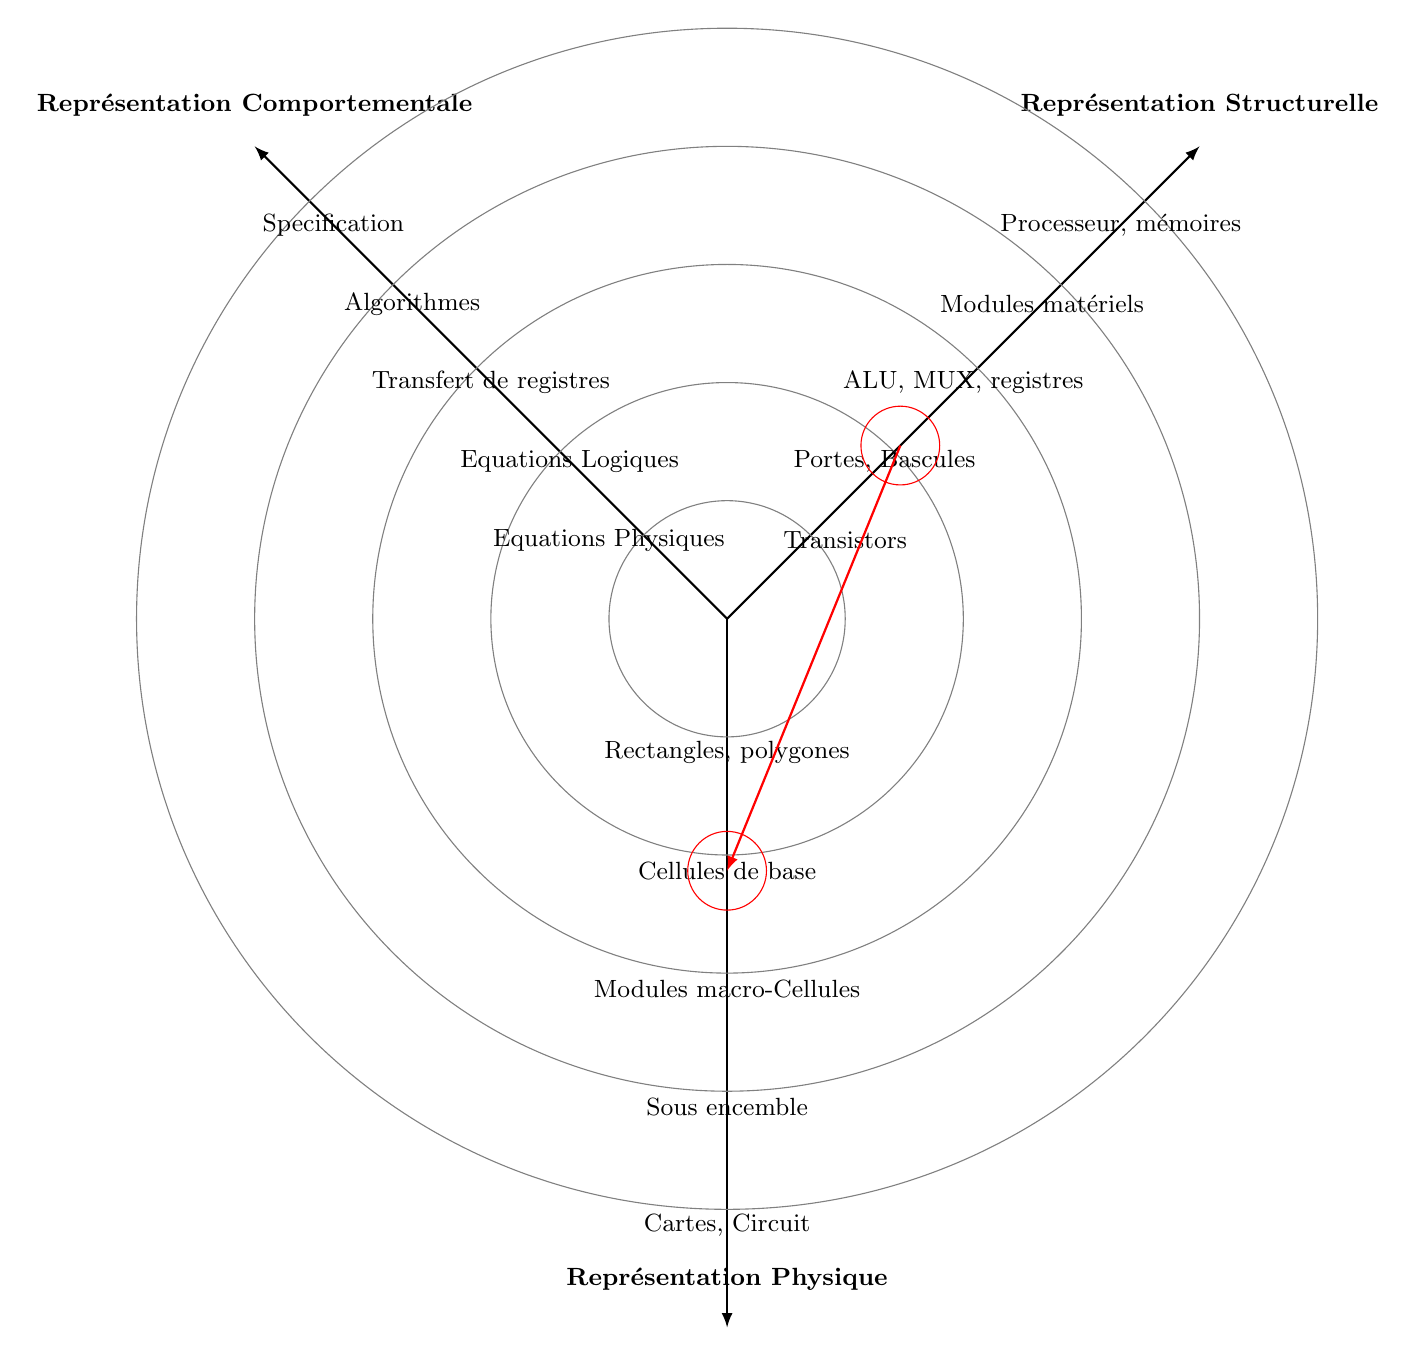
\begin{tikzpicture}[
    axis/.style={thick, -latex},
    font=\small
]

% Appliquer une rotation de 180°
\begin{scope}

% Définir les coordonnées pour les trois axes
\coordinate (O) at (0,0); % Centre
\coordinate (B) at (-6,6); % Axe Behavioral (inversé en Y)
\coordinate (S) at (6,6);  % Axe Structural (inversé en Y)  
\coordinate (P) at (0,-9);   % Axe Physical (inversé en Y)

% Dessiner les axes
\draw[axis] (O) -- (B) node[at end, yshift=15pt] {\textbf{Représentation Comportementale}};
\draw[axis] (O) -- (S) node[at end, yshift=15pt] {\textbf{Représentation Structurelle}};
\draw[axis] (O) -- (P) node[at end, below, yshift=25pt] {\textbf{Représentation Physique}};

% Cercles concentriques
\draw[gray, thin] (O) circle (1.5);
\draw[gray, thin] (O) circle (3);
\draw[gray, thin] (O) circle (4.5);
\draw[gray, thin] (O) circle (6);
\draw[gray, thin] (O) circle (7.5);

% Niveaux sur l'axe Behavioral (côté gauche) - inversés en Y
\node[align=center] at (-1.5,1) {Equations Physiques};
\node[align=center] at (-2,2) {Equations Logiques};
\node[align=center] at (-3,3) {Transfert de registres};
\node[align=center] at (-4,4) {Algorithmes};
\node[align=center] at (-5,5) {Specification};

% Niveaux sur l'axe Structural (côté droit) - inversés en Y
\node[align=center] at (1.5,1) {Transistors};
\node[align=center] at (2,2) {Portes, Bascules};
\node[align=center] at (3,3) {ALU, MUX, registres};
\node[align=center] at (4,4) {Modules matériels};    
\node[align=center] at (5,5) {Processeur, mémoires};

% Niveaux sur l'axe Physical (bas) - inversés en Y
\node[align=center] at (0,-1.7) {Rectangles, polygones};
\node[align=center] at (0,-3.2) {Cellules de base};
\node[align=center] at (0,-4.7) {Modules macro-Cellules};
\node[align=center] at (0,-6.2) {Sous encemble};
\node[align=center] at (0,-7.7) {Cartes, Circuit};

\draw[red, thin] (2.2,2.2) circle (0.5);
\draw[red, thin] (0,-3.2) circle (0.5);

\draw[red, thick, -latex] (2.2,2.2) -- (0,-3.2);

\end{scope}

\end{tikzpicture}
   }
\caption{Diagramme en Y - Action de routage}
\label{fig:diagramme_y_synthese}
\end{figure}

\subsection{Interface Microprocesseur}

Après l'étape de \textbf{synthèse}, nous pouvons nous intéresser à l'assignation des ressources 
matérielles du système.\\
Pour cela, nous utilisons le logiciel \textbf{Vivado} (étant donné que les outils de HDL n'étaient 
pas disponibles le jour du TP), qui permet de générer un schéma RTL ainsi qu'une vue du routage 
associé à l'interface microprocesseur.
\newline

Dans un premier temps, Nous allons resynthétiser le design afin d'obtenir le schéma RTL.
Ce schéma, présenté ci-dessous, illustre les ressources logiques utilisées pour implémenter 
l'interface microprocesseur.
\newline

\resizebox{\textwidth}{!}{%
    \includegraphics[angle=-90]{images/Routage/pdf_recadre_recadre.pdf}%
}

\vspace{10pt}

Par la suite, nous pouvons également observer la synthèse matérielle réalisée sur Vivado, qui 
transforme les ressources logiques en ressources matérielles pour le FPGA.
\newline

\begin{figure}[H]
    \centering
    \includegraphics[width=0.8\linewidth]{images/Routage/schematic_RTL_VIVADO_recadre.pdf}
    \caption{Synthèse matérielle Vivado}
    \label{fig:rout_general}
\end{figure}

Cette synthèse nous montre que la logique est transformée en ressource matérielle, notamment des 
LUT (Look-Up Tables) et des Flip-Flops, qui sont les éléments de base pour implémenter la logique 
dans un FPGA.
\newline

Les \textbf{LUT} (Look-Up Tables), éléments fondamentaux d'un FPGA, peuvent être considérées comme 
des portes logiques programmables capables de réaliser toute fonction combinatoire. 
Elles constituent la base de l'implémentation matérielle et offrent une vision schématique complète 
du système.  
\newline

Prenons l'exemple d'une \textbf{LUT3} :  

\begin{figure}[H]
    \centering
    % Première image
    \begin{subfigure}[b]{0.55\linewidth}
        \centering
        \includegraphics[width=\linewidth]{images/Routage/LUT_EXEMPLE.png}
        \caption{Exemple de LUT}
        \label{fig:lut_exemple}
    \end{subfigure}
    \hfill
    % Deuxième image
    \begin{subfigure}[b]{0.25\linewidth}
        \centering
        \includegraphics[width=\linewidth]{images/Routage/TABLE_LUT.png}
        \caption{Table de vérité associée}
        \label{fig:table_lut}
    \end{subfigure}
    \caption{Illustration d'une LUT et de sa table de vérité}
    \label{fig:lut_complete}
\end{figure}

Grace à la table de vérité de la LUT nous remarquons que cette LUT3 implémente une fonction logique ET à trois entrées.
\newline

\begin{figure}[H]
    \centering
    \includegraphics[width=0.8\linewidth]{images/Routage/Mux_Tris_Vivado.png}
    \caption{Synthèse Logique Vivado}
    \label{fig:rout_general}
\end{figure}

Nous observons également la présence de la partie opérative de l'interface Microprocesseur.
\newline

\medskip

La suite du flot de conception consiste à lancer l'\textbf{implémentation} du système afin d'obtenir le routage complet. 
Vivado propose alors une vue générale du FPGA, mettant en évidence ses différentes zones fonctionnelles :  

\begin{figure}[H]
    \centering
    \includegraphics[width=0.8\linewidth]{images/Routage/Rout_1.png}
    \caption{Slice du FPGA après routage}
    \label{fig:rout_general}
\end{figure}

En effectuant un zoom, il est possible de constater que le système a été implémenté dans la zone \textbf{0} du FPGA. 
Nous observons que la zone située à gauche correspond aux entrées de chaque variable, 
celles-ci étant toutes reliées à des \textbf{buffers}.

\begin{figure}[H]
    \centering
    % Première image (anciennement deuxième)
    \begin{subfigure}[b]{0.45\linewidth}
        \centering
        \includegraphics[width=\linewidth]{images/Routage/Rout_2.png}
        \caption{Localisation du système dans la zone 0 du FPGA}
        \label{fig:rout_zone0}
    \end{subfigure}
    \hfill
    % Deuxième image (anciennement première)
    \begin{subfigure}[b]{0.50\linewidth}
        \centering
        \includegraphics[width=\linewidth]{images/Routage/buff.png}
        \caption{Buffer associé à nCS}
        \label{fig:buff_ncs}
    \end{subfigure}
    \caption{Vue du système routé et des buffers associés sur le FPGA}
    \label{fig:rout_buff}
\end{figure}



Un zoom encore plus détaillé permet d'observer le câblage interne des ressources identifiées lors de la synthèse.  
Par exemple, une \textbf{LUT3} est câblée de la manière suivante :  

\begin{figure}[H]
    \centering
    % Première image
    \begin{subfigure}[b]{0.35\linewidth}
        \centering
        \includegraphics[width=\linewidth]{images/Routage/Rou_3.png}
        \caption{Connexion interne d'une LUT3}
        \label{fig:rout_lut3a}
    \end{subfigure}
    \hfill
    % Deuxième image
    \begin{subfigure}[b]{0.55\linewidth}
        \centering
        \includegraphics[width=\linewidth]{images/Routage/Rou_4.png}
        \caption{Schéma détaillé du câblage LUT3}
        \label{fig:rout_lut3b}
    \end{subfigure}
    \caption{Exemple de routage d'une LUT3 dans le FPGA}
    \label{fig:rout_lut3}
\end{figure}

\medskip

Le résultat final est une représentation complète et hiérarchisée du système, directement mappée sur le FPGA. 
\textbf{Vivado} offre ainsi la possibilité de visualiser l'ensemble du flot, depuis la description logique RTL jusqu'au routage physique détaillé.  

En résumé, la conception suit une progression en trois étapes :  
\begin{itemize}
    \item la \textbf{synthèse} génère une description logique optimisée du système (LUT, registres, blocs fonctionnels) ;  
    \item le \textbf{placement} attribue ces ressources aux cellules physiques du FPGA ;  
    \item le \textbf{routage} établit les interconnexions nécessaires au bon fonctionnement du circuit.  
\end{itemize}

Cette approche permet de passer d'une description abstraite en langage HDL à une implémentation matérielle 
concrète, où chaque fonction logique est traduite en ressources physiques. 
Vivado fournit alors une vision globale et détaillée du FPGA, allant de la logique combinatoire jusqu'au câblage interne des composants.

\subsection{FIFO}

Après l'étape de synthèse, nous pouvons nous intéresser à l'assignation des ressources 
matérielles du système FIFO, qui permet de générer un schéma de ressources utilisées pour l'implémentation
de la FIFO.
\newline

Voici le schéma RTL de la FIFO implémentée :

\begin{figure}[H]
    \centering
    \resizebox{\textwidth}{!}{%
        \rotatebox{-90}{\includegraphics[width=0.9\linewidth]{images/Routage/fifo_viv_recadre.pdf}}
    }
    \caption{Schéma Vivado de la FIFO - Vue générale}
    \label{fig:RTL_FIFO}
\end{figure}

\begin{figure}[H]
    \centering
    \resizebox{\textwidth}{!}{%
        \includegraphics[width=0.9\linewidth]{images/Routage/Zoom_FIFI_viv.png}
    }
    \caption{Schéma Vivado de la FIFO - Vue détaillée}
    \label{fig:RTL_FIFO}
\end{figure}

On identifie clairement l'architecture dual-port de la FIFO avec ses \textbf{registres} organisés en matrice 9x8 bits 
pour le stockage des données. La gestion des adresses est assurée par un \textbf{compteur 4 bits} implémenté avec des bascules 
\textbf{FDCE} et des \textbf{LUT} qui calculent les incréments et les conditions de débordement. Les entrées-sorties sont conditionnées 
par des \textbf{buffers} pour l'interface avec l'extérieur du FPGA, tandis qu'un \textbf{buffer global} distribue 
l'horloge à l'ensemble du système. La logique de contrôle, répartie dans de multiples \textbf{LUT2 à LUT6}, gère simultanément les 
opérations d'écriture via \texttt{OctetRecu\_WR} et de lecture via \texttt{OctetLu\_RD} tout en maintenant la cohérence des pointeurs 
et en générant les signaux de statut.
\newline

\subsection{EtatInterne}

Après l'étape de synthèse, nous pouvons nous intéresser à l'assignation des ressources
matérielles du système EtatInterne, qui permet de générer un schéma de ressources utilisées pour l'implémentation
de l'EtatInterne.
\newline

Voici le schéma RTL de l'EtatInterne implémentée :

\begin{figure}[H]
    \centering
    \resizebox{\textwidth}{!}{%
        \rotatebox{-90}{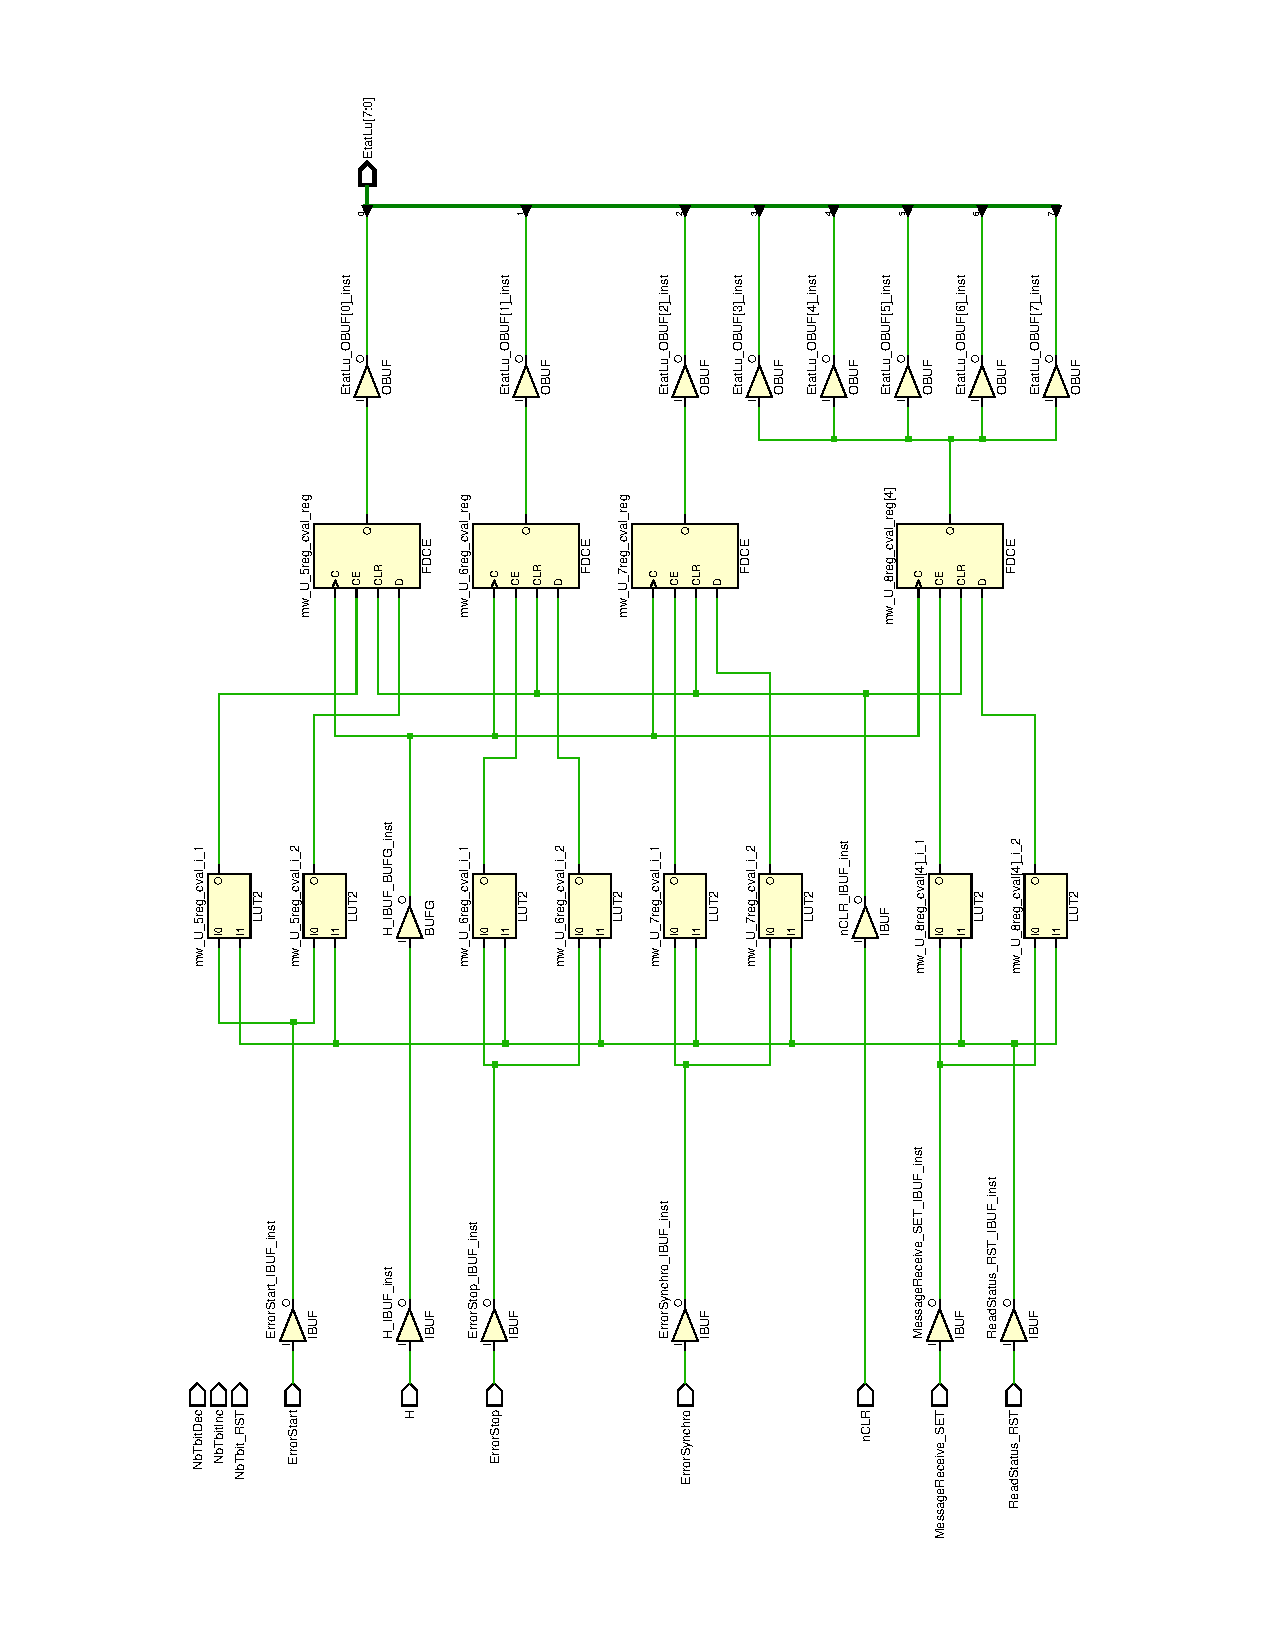
\includegraphics{images/Routage/InternalState_viv_recadre.pdf}}
    }
    \caption{Schéma RTL de l'EtatInterne}
    \label{fig:RTL_EtatInterne}
\end{figure}

On identifie clairement un ensemble de \textbf{bascules D)} organisées pour mémoriser les différents états du système. 
Ces bascules sont pilotées par une logique combinatoire implémentée via des \textbf{LUT }, qui définissent les 
transitions d'état en fonction des signaux de commande et des conditions internes. Les entrées sont conditionnées par des 
\textbf{buffers} afin d'isoler et d'adapter les signaux externes aux ressources internes du FPGA, assurant ainsi une 
intégrité électrique et temporelle. En sortie, des \textbf{buffers} sont utilisés pour transmettre l'état courant vers les blocs suivants.
\newline

Dans ce schéma nous avons des signaux non, reliées surement une erreur de Vivado. Normalement ces signaux devraient être connectés à une LUT dont la 
table de vérité permettrait de réaliser la fonction \textbf{DECODE}, qui permet de choisir entre incrémentation et décrémentation du compteur du nombre d'octet. .
\newline 

\subsection{Interface Reception Lin}

Cette Phase n'étant pas réellement necessaire pour la validation du projet, nous avans décider de juste de faire l'implémentation du projet global, et non de montrer les ressources de chacune des sections.
\newline

Donc comme l'interface microprocesseur, nous avons fait l'implémentation de l'interface de réception LIN ( global ) et voici le résultat du routage :

\begin{figure}[H]
    \centering
    \includegraphics[width=0.9\linewidth]{images/Routage/impl_schematic_recadre.pdf}
    \caption{Schéma Implémentation Matérielle Reception LIN}
    \label{fig:Impl_RTL_Shematic_Reception}
\end{figure}


Dans celui ci, nous pouvons observer les différentes ressources matérielles utilisées pour l'implémentation de l'interface de réception LIN.
notamment les LUTs, les Flip-Flops, et les autres composants logiques.
\newline

Ce schéma étant dense et complexe, nous n'allons pas détailler chaque partie, mais il illustre bien comment les ressources matérielles sont utilisées pour réaliser les fonctions de l'interface de réception LIN.
Voici un exemple de LUT retrouvée dans le routage de l'interface de réception Trame : 


\begin{figure}[H]
    \centering
    \includegraphics[width=0.9\linewidth]{images/Routage/ZOOM_Imple.png}
    \caption{Schéma Implémentation Matérielle Reception LIN Zoom 1}
    \label{fig:Impl_ZOOM_1_RTL_Shematic_Reception}
\end{figure}


Dans ce zoom, nous pouvons voir une LUT spécifique utilisée dans le routage de l'interface de réception LIN. La présentation d'un LUT est plus détaillée 
dans la section précédente.
\newline

Voici également le routage global de l'interface de réception LIN sur le FPGA :


\begin{figure}[H]
    \centering
    \includegraphics[width=0.9\linewidth]{images/Routage/RoutageFinal.png}
    \caption{Slice du FPGA après routage de l'interface de réception LIN}
    \label{fig:Routage_Shematic_Reception}
\end{figure}


Pareillement, cette représentation étant dense, nous n'allons pas détailler chaque partie, mais elle illustre comment les ressources matérielles sont utilisées pour réaliser les fonctions de l'interface de réception LIN.
\newline

\begin{figure}[H]
    \centering
    \includegraphics[width=0.9\linewidth]{images/Routage/RoutageFinal_Zoom.png}
    \caption{Slice du FPGA après routage de l'interface de réception LIN - Zoom sur Zone 0}
    \label{fig:Routage_ZOOM_1_Shematic_Reception}
\end{figure}

A la fin du projet nous avons la possibilité de voir l'utilisation des ressources du FPGA par Vivado.

\begin{table}[h!]
\centering
\resizebox{\textwidth}{!}{%
\begin{tabular}{|l|c|c|c|c|c|c|}
\hline
\textbf{Name} & \textbf{Slice LUTs (20800)} & \textbf{Slice Registers (41600)} & 
\textbf{Slice (8150)} & \textbf{LUT as Logic (20800)} & 
\textbf{Bonded IOB (106)} & \textbf{BUFCTRL (32)} \\ \hline
RecepteurLin & 140 & 132 & 55 & 140 & 15 & 1 \\ \hline
\end{tabular}%
}
\caption{Utilisation des ressources FPGA pour le module \texttt{RecepteurLin}}
\label{tab:recepteurlin}
\end{table}

